\section{CAN-CNA}
\subsection{Généralités}

Dans le monde réel, l'information est généralement représentée sous forme de 
signaux analogiques. Ces signaux sont le plus souvent électriques et leur forme 
reflète en continu l'évolution d'une grandeur physique.\par

Un signal analogique est donc une représentation continue dans le temps, dont un 
ou plusieurs paramètres — typiquement l’amplitude ou la fréquence — sont 
proportionnels à une grandeur physique d’origine. Voici quelques exemples 
classiques de grandeurs analogiques ~:

\begin{itemize}
    \item \textbf{L’intensité lumineuse} ~: convertie en tension électrique par un photodétecteur.
    \item \textbf{La pression acoustique} ~: convertie en signal électrique par un microphone.
    \item \textbf{La température} ~: convertie en tension par une thermistance ou un capteur analogique.
\end{itemize}

\textbf{\sffamily Illustration ~: codage d’une ligne d’image}

Prenons l’exemple d’un balayage d’image. L’intensité lumineuse captée ligne par 
ligne est convertie en une tension analogique proportionnelle. À titre 
d’illustration ~:

\begin{itemize}
    \item Au début de la ligne, la tension est nulle (\SI{0}{\volt}) ~: cela correspond à une zone sombre (noir).
    \item À la fin de la ligne, la tension atteint \SI{0.7}{\volt} ~: cela correspond à une zone très claire (blanc).
\end{itemize}

Cette variation continue de la tension en fonction du temps représente 
fidèlement le dégradé d’intensité lumineuse de la ligne d’image.

\vspace{0.5cm}
\textbf{\sffamily Représentation schématique ~:}

\begin{minipage}{0.30\textwidth}
    \centering
    
\begin{tikzpicture}
        \draw[left color=black,right color=white] (0,0) rectangle (4,4);
    \end{tikzpicture}
\end{minipage}
\begin{minipage}{0.33\textwidth}
    \centering
    \begin{tikzpicture}
        \draw[line width=1mm, -{>[length=4mm]}] (0,2) -- (3,2);
    \end{tikzpicture}    
\end{minipage}
\begin{minipage}{0.33\textwidth}
    \centering
    \resizebox{\linewidth}{!}{%
    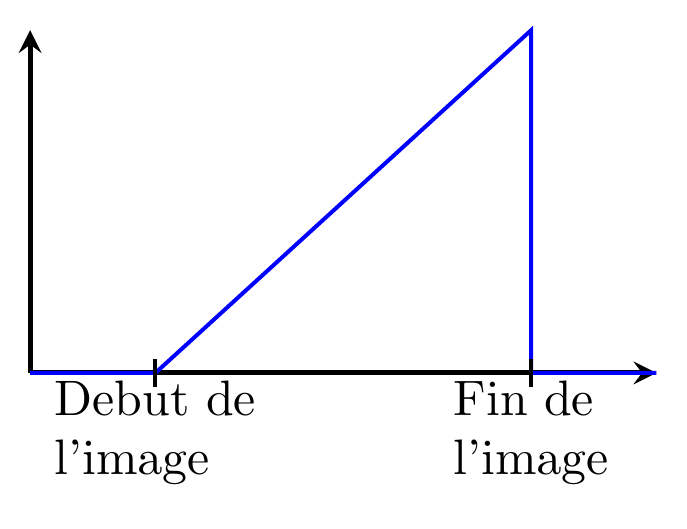
\begin{tikzpicture}[scale=1.8]
        \begin{axis}[
            width=6cm,height=4cm,
            axis y line=center,
            axis x line=middle, 
            ticks=none,
            axis line style={line width=1pt},
            clip=false,
        ]
        \addplot+[mark=none, thick,] coordinates
        {(0,0) (0.25,0) (1,0.5) (1,0) (1.25,0)};
        \draw[-, thick, black] (axis cs:0.25,-0.02) -- (axis cs:0.25,0.02) node[below,pos=0.9,align=left] {Debut de\\l'image};
        \draw[-, thick, black] (axis cs:1,-0.02) -- (axis cs:1,0.02) node[below,pos=0.9,align=left] {Fin de\\l'image};
        
    \end{axis}
    \end{tikzpicture}
    }
\end{minipage}

\vspace{0.2cm}

\textit{(Note ~: L’illustration ci-dessus montre l’évolution temporelle d’une 
tension analogique correspondant au balayage d’une ligne d’image du noir 
vers le blanc.)}

La plupart des grandeurs physiques que nous mesurons existent sous forme \textbf{analogique} ~: température, vitesse, position, pression, force, etc. Un signal analogique se caractérise par un \textbf{nombre infini de points de mesure}. Cela signifie que ~:
\begin{itemize}
    \item L'information est \textbf{continue} dans le temps.
    \item L'information est \textbf{continue} en amplitude.
\end{itemize}

Un signal analogique typique peut être représenté par la courbe ci-dessous ~:

\begin{center}
    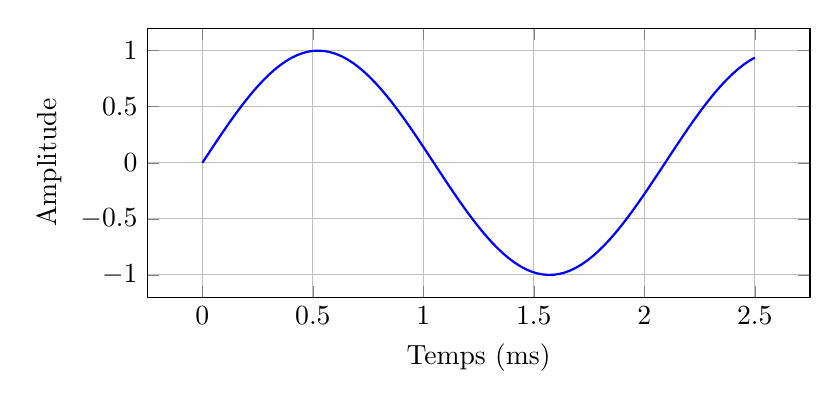
\begin{tikzpicture}
        \begin{axis}[
            xlabel={Temps (ms)},
            ylabel={Amplitude},
            grid=major,
            width=10cm, height=5cm,
            domain=0:2.5, samples=100,
            ytick={-2,-1.5,-1,-0.5,0,0.5,1,1.5,2}
        ]
            \addplot[blue, thick] {sin(deg(3*x))};
        \end{axis}
    \end{tikzpicture}
\end{center}

Comme le montre ce graphique, un signal analogique possède une infinité de 
valeurs et une infinité de points de mesure.


Le processus de \textbf{numérisation} consiste à transformer un signal analogique 
en une \textbf{suite de valeurs numériques} qui décrivent ses variations. 
Puisqu'il est impossible de stocker une infinité de points, il est nécessaire de ~:
\begin{itemize}
    \item \textbf{Limiter} le nombre de points de mesure, c'est l’opération d’\textbf{échantillonnage}.
    \item \textbf{Coder} chaque échantillon avec un nombre fini de chiffres.
\end{itemize}


L’échantillonnage consiste donc à prendre un certain nombre de points 
représentatifs du signal analogique. Chaque point est ensuite \textbf{quantifié} 
et \textbf{codé} en une valeur numérique exploitable par un système numérique.
\begin{figure}[H]
    \centering
    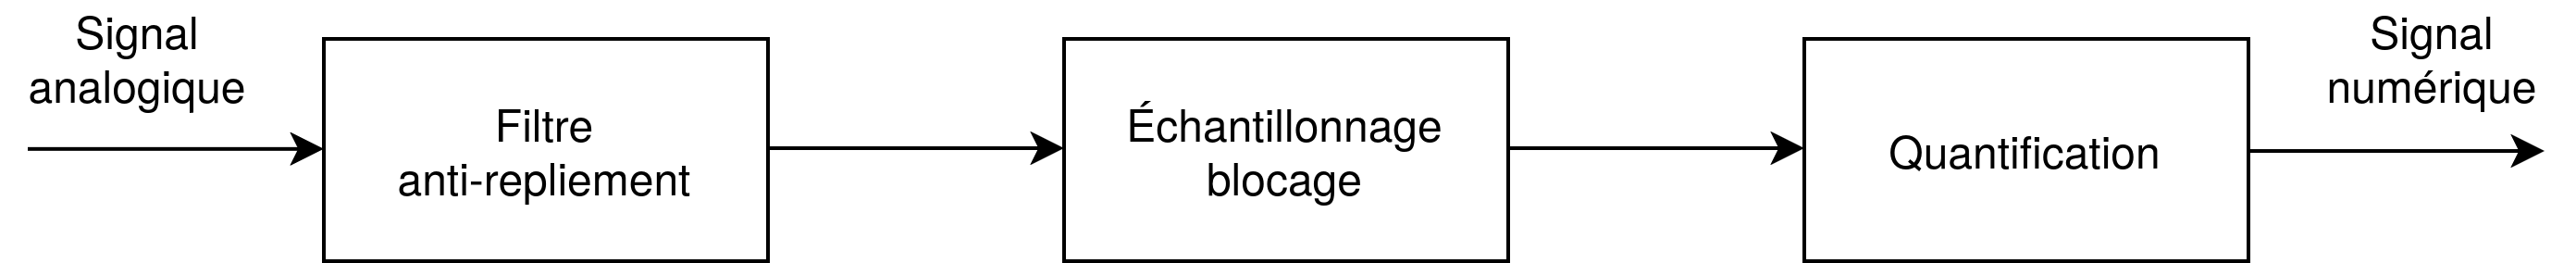
\includegraphics[width=0.8\textwidth]{can}
    \caption{Chaine de conversion numérique-analogique}
    \label{figCna}
\end{figure}

\`A l’inverse, un signal numérique peut être transformé en un signal analogique 
grâce à un \textbf{convertisseur numérique-analogique} (CNA). Ce processus est
appelé \textbf{conversion numérique-analogique} et consiste à reconstituer le
signal analogique à partir des valeurs numériques. Le CNA effectue une
\textbf{interpolation} entre les points numériques pour créer un signal analogique
continu. Il est important de noter que la qualité de la conversion dépend de la
fréquence d'échantillonnage et de la résolution du convertisseur. Un échantillonnage
trop faible peut entraîner une perte d'information, tandis qu'une résolution
insuffisante peut introduire des erreurs dans la représentation du signal
analogique. La figure \ref{fig:chaine-cna} illustre le processus de conversion
numérique-analogique. Le signal numérique est d'abord échantillonné, puis
quantifié et enfin converti en un signal analogique continu.
\begin{figure}[H]
    \centering
    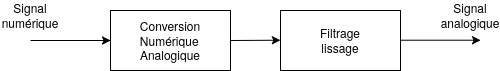
\includegraphics[width=0.8\textwidth]{cna}
    \caption{Chaine de conversion analogique-numérique}
    \label{figChaineCna}
\end{figure}

\subsection{\'Echantillonnage-Blocage}

Exemple, on veut num\'eriser la fonction suivante ~:
\begin{figure}[H]
    \centering
    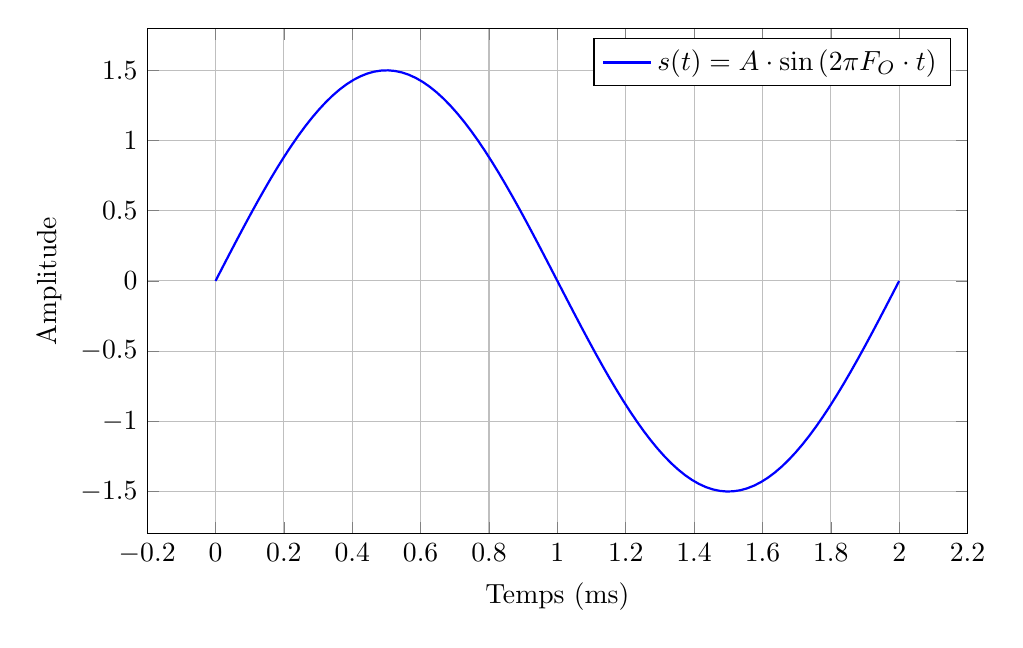
\begin{tikzpicture}
        \begin{axis}[
            xlabel={Temps (ms)},
            ylabel={Amplitude},
            grid=major,
            width=12cm, height=8cm,
            domain=0:2, samples=100,
            ytick={-2,-1.5,-1,-0.5,0,0.5,1,1.5,2}
        ]
            \addplot[blue, thick] {1.5*sin(deg(2*pi*0.5*x))};
            \legend{\(s(t)=A\cdot\sin{\left(2\pi F_{O}\cdot t\right)}\)};
        \end{axis}
    \end{tikzpicture}
    \caption{Signal analogique}
    \label{figSignalAnalogique}
\end{figure}

La première étape consiste à échantillonner le signal analogique. Pour cela, on
prend des échantillons à intervalles réguliers. Par exemple, on peut choisir de
prélever un échantillon tous les \(T_e\) (ici \SI{0.125}{\ms}). La fréquence
d'échantillonnage est donc \(F_e=\frac{1}{T_e}\). Dans notre exemple, on a ~:
\[
    F_e = \frac{1}{T_e} = \frac{1}{0.125} = 8 \text{ kHz}
\]
\begin{figure}[H]
    \centering
    \begin{tikzpicture}
        \begin{axis}[
            xlabel={Temps (ms)},
            ylabel={Amplitude},
            grid=major,
            width=12cm, height=8cm,
            domain=0:2, samples=100,
            ytick={-2,-1.5,-1,-0.5,0,0.5,1,1.5,2},
            xtick={0,0.5,1,1.5,2}
        ]
            \addplot[blue, thick] {1.5*sin(deg(2*pi*0.5*x))};
            \legend{\(s(t)=A\cdot\sin{\left(2\pi F_{O}\cdot t\right)}\)};

            \addlegendimage{blue, thick, mark=*, mark options={color=red, scale=1.5}} \addlegendentry{Echantillon}
            
            \pgfplotsinvokeforeach {0,0.125,...,2} {
                \addplot[red, mark=*, only marks, mark options={scale=1.5}] 
                    coordinates {
                        (#1, {1.5*sin(deg(2*pi*0.5*#1)))})
                    };
                \addplot[dashed, samples=50, smooth,domain=0:6,gray] 
                    coordinates {
                        (#1, {1.5*sin(deg(2*pi*0.5*#1)))}) (#1,0)
                    };
                \closedcycle;
            }
            \addplot[dashed, samples=50, smooth,gray] coordinates {(0.5,0) (0.5,-0.25)};
            \addplot[dashed, samples=50, smooth,gray] coordinates {(0.625,0) (0.625,-0.25)};
            \draw[<->, thick, RoyalPurple] (axis cs:0.5,-0.22) -- (axis cs:0.625,-0.22) node[below,pos=0.5,align=center, RoyalPurple] {\(T_e\)};
        \end{axis}
    \end{tikzpicture}
    \caption{Signal analogique échantillonné}
    \label{figSignalEchantillonne}
\end{figure}

On obtient ainsi une série de points discrets, qui représentent le signal
analogique à des instants précis. Ces points sont appelés \textbf{échantillons}.
Ensuite, on doit \textbf{bloquer} le signal entre chaque échantillon. Cela signifie
que l'on maintient la valeur de chaque échantillon constant jusqu'au prochain
échantillon. Le signal résultant est donc une série de segments horizontaux,
représentant la valeur de chaque échantillon. Ce processus est souvent appelé
\textbf{signal bloqué} ou \textbf{signal échantillonné et bloqué}. Il est important
de noter que le signal bloqué ne représente pas fidèlement le signal analogique
d'origine, car il ne conserve que les valeurs des échantillons et ignore les
variations entre eux. Cependant, il est plus facile à traiter par un système
numérique, car il est discret dans le temps et l'amplitude.

\begin{figure}[H]
    \centering
    \begin{tikzpicture}
        \begin{axis}[
            xlabel={Temps (ms)},
            ylabel={Amplitude},
            grid=major,
            width=12cm, height=8cm,
            domain=0:2, samples=100,
            ytick={-2,-1.5,-1,-0.5,0,0.5,1,1.5,2},
            xtick={0,0.5,1,1.5,2}
        ]
            \addplot[blue, thick] {1.5*sin(deg(2*pi*0.5*x))};
            \legend{\(s(t)=A\cdot\sin{\left(2\pi F_{O}\cdot t\right)}\)};
            
            \addlegendimage{blue, thick, mark=*, mark options={color=red, scale=1.5}} \addlegendentry{Echantillon}
            \addlegendimage{red, thick} \addlegendentry{Signal bloqué}

            \pgfplotsinvokeforeach {0,0.125,...,2} {
                \addplot[red, mark=*, only marks, mark options={scale=1.5}] 
                    coordinates {
                        (#1, {1.5*sin(deg(2*pi*0.5*#1)))})
                    };
                \addplot[dashed, samples=50, smooth,domain=0:2,gray] 
                    coordinates {
                        (#1, {1.5*sin(deg(2*pi*0.5*#1)))}) (#1,0)
                    };
                \ifdim #1 pt<2pt
                \addplot[red, thick, samples=50, smooth,domain=0:2] 
                    coordinates {
                        (#1, {1.5*sin(deg(2*pi*0.5*#1)))}) (#1+0.125,{1.5*sin(deg(2*pi*0.5*#1)))})
                    };
                    \addplot[red, thick, samples=50, smooth,domain=0:2]
                        coordinates {
                            (#1+0.125, {1.5*sin(deg(2*pi*0.5*#1))})
                            (#1+0.125, {1.5*sin(deg(2*pi*0.5*(#1+0.125)))})
                        };
                \fi
            \closedcycle;
            }
            \addplot[dashed, samples=50, smooth,gray] coordinates {(0.5,0) (0.5,-0.25)};
            \addplot[dashed, samples=50, smooth,gray] coordinates {(0.625,0) (0.625,-0.25)};
            \draw[<->, thick, RoyalPurple] (axis cs:0.5,-0.22) -- (axis cs:0.625,-0.22) 
            node[below,pos=0.5,align=center, RoyalPurple] {\(T_e\)};
        \end{axis}
    \end{tikzpicture}
    \caption{Signal analogique échantillonné et bloqué}
    \label{figSignalEchantillonneBloque}
\end{figure}


Un échantillonneur-bloqueur peut être réalisé à l'aide des composants suivants ~:
\begin{itemize}
    \item Un interrupteur commandé par un signal TTL (signal carré prenant deux valeurs ~: 0~V et 5~V), appelé \textit{signal d'horloge},
    \item Un condensateur,
    \item Une résistance montée en parallèle avec le condensateur.
\end{itemize}

\begin{figure}[H]
    \centering
    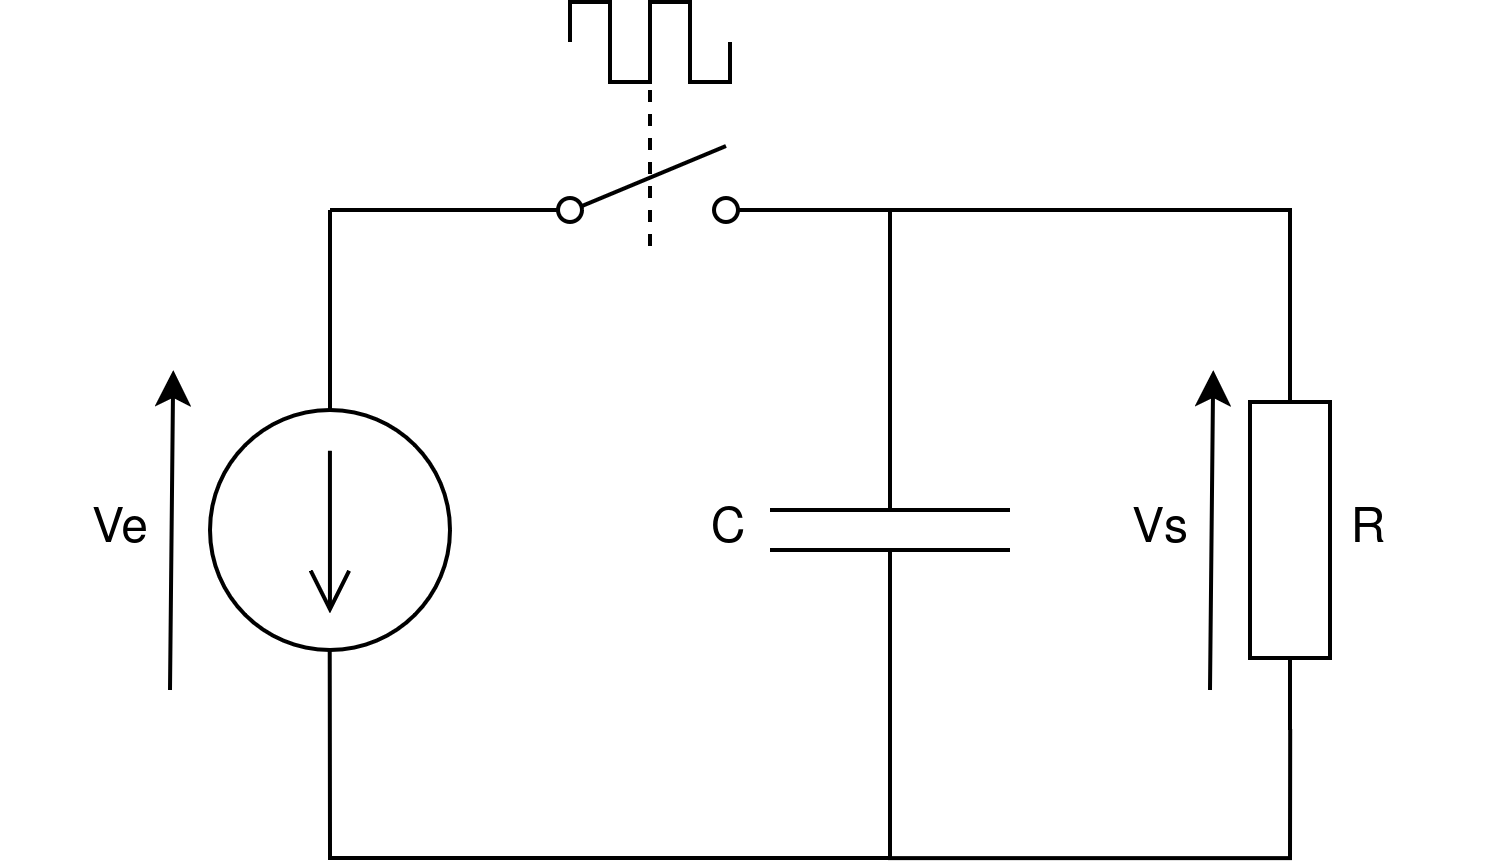
\includegraphics[width=0.8\textwidth]{echant-bloc-circ}
    \caption{\'Echantillonneur-bloqueur}
    \label{figEchantillonneur}
\end{figure}

Ce circuit est utilisé dans la chaîne d'acquisition analogique-numérique, notamment avant un convertisseur analogique-numérique (CAN).

\paragraph{Fonctionnement ~:}
On distingue deux états de fonctionnement en fonction de l'état de l'interrupteur ~:

\begin{enumerate}[(a)]
    \item \textbf{Interrupteur fermé ~:} Le condensateur suit la tension d'entrée. La tension de sortie est donc égale à la tension d'entrée ~:\\
    \[
        V_s = V_e
    \]
    
    \item \textbf{Interrupteur ouvert ~:} Le condensateur est isolé de l'entrée et conserve sa charge. La tension de sortie reste constante ~:\\
    \[
        V_s = \text{constante}
    \]
\end{enumerate}